%\newgeometry{left=5cm, right=4cm,bottom=4cm, top=4cm}
\newgeometry{left=4.2cm, right=3.9cm,bottom=4cm} %, top=3cm}
\chapter{Reconstruction of Physics Objects}\label{chap:obj} \vspace{2cm}

The raw ATLAS  data containing  signals of all detector read-out channels, need to
undergo  several reconstruction steps before they can be analyzed. The event reconstruction software is 
implemented in the ATLAS  software framework ATHENA~\cite{Athena}.
% which allow for reconstruction and 
%identification of various objects corresponding to physics particles traversing the detector.
This chapter describes the procedure for the  reconstruction  of physics objects relevant for the
analysis presented in this thesis.
For a detailed overview of the ATLAS detector reconstruction software  see~\cite{AtlasCSCBook}. 

\restoregeometry
\clearpage

\section{Reconstruction of Charged Particle Tracks}
The reconstruction of charged particles tracks and interaction vertices is based on the measurements in the inner detector
which allow  for the reconstruction of tracks within the pseudorapidity range of $|\eta| < 2.5$. 
A track is characterized by its four-momentum vector and two impact parameters: $d_0$, i.e.,  the distance 
of closest approach between the track and the interaction point in the transverse plane and $z_0$, i.e.
the $z$ coordinate of the track calculated at the same point of closest approach. 


Tracks are reconstructed  by the inner detector track reconstruction software~\cite{IDtracking}.
First raw data from the pixel and SCT detectors are transformed into three-dimensional space points 
(so called ``hits''), while the  TRT detector information is translated into drift circles. 
Subsequently, track seeds are formed from a combination of space-points in the three pixel layers and the first SCT layer. These
seeds are then extrapolated through the SCT to form track candidates  from all hits on the track path. The track candidates are obtained by a 
fit trough all hits using a \emph{Kalman filter} algorithm~\cite{Kalman}. Ambiguities in the  association of the hits to the track 
are resolved by this fitting procedure and  tracks produced by a random association of hits are rejected. The selected tracks are then 
extrapolated to the TRT and finally refitted using the full information of all three tracking detectors. 
In order to  improve the tracking efficiency for secondary tracks  from photon conversion or decays 
of long-lived particles (like kaons), a complementary algorithm~\cite{IDtracking} searches 
for unassociated track segments in the TRT, these segments are then extrapolated towards the SCT and the pixel detector in
a similar manner as in the default algorithm. All tracks with $\pt > 100$ MeV are considered for physics
analysis.


\section{Vertex Reconstruction}
The vertex reconstruction algorithm and its performance are described in detail in~\cite{AtlasCSCBook,VertexPerf} and
only briefly summarized here.
%say good tracks
The vertex finding algorithm selects a set of well reconstructed tracks and generates
a vertex  seed according to the average value of the tracks $z$ coordinate. The $z$ coordinate of the tracks
is computed relative to  the expected average position of the collision point. 
An \emph{adaptive vertex fitting} algorithm~\cite{Vertex} determines the vertex position based on the vertex seed  and on the 
tracks around it via a $\chi^2$ fit.  Based on this fit, tracks that are incompatible with the found vertex by more than seven standard deviations
are used to seed the next vertex. The procedure is performed iteratively until either all tracks are associated to a vertex
 or no additional vertex can be found.
The performance of this procedure depends  on the expected position of the average interaction point which is monitored 
during LHC data taking and is computed in intervals of a  few minutes as described in~\cite{beamspot}.

The vertex with the largest sum of transverse momentum of all associated tracks is identified as the \emph{primary vertex} (PV), 
corresponding to  the interaction point of the hard scattering process in the event. All  other vertices in the event
are assumed to result from minimum bias interactions and are called \emph{pile-up} vertices.
In data recorded during 2012, there were on  average  21 multiple interactions  occurring per bunch crossing.
Such a high vertex multiplicity strongly affects the ambient energy density in the event,
such that an accurate pile-up description in simulation is  crucial for the modelling of physics processes. In ATLAS, 
events are simulated assuming various pile-up conditions and weighted such to reproduce  the observed 
average number of interactions per bunch crossing.


\section{Electron Reconstruction and Identification} \label{sec:elec}
Electron are reconstructed and identified by combining EM calorimeter and inner detector measurements.
The corresponding dedicated  algorithm is described in~\cite{electronAlgo}.
The electron candidate is reconstructed as a  clusters of EM calorimeter cells which is matched to a track
in the inner detector. Special care during the matching is taken to account for 
Bremsstrahlung losses of the charged particle.
%Once an electromagnetic shower in the calorimeter is 
%found to match with one or more tracks, the combination of those is considered as an electron candidate.  
The electron energy is computed as 
a weighted average between the cluster energy and the track momentum. Several corrections are applied to
take into account energy losses in the material of the inner detector and effect of electromagnetic shower 
leakage. The electron direction is defined by the corresponding track parameters. 

Further identification criteria are applied to electron candidates to reduce contaminating contribution of 
photon conversions and hadronic jets. Three different identification criteria are provided based on a multi-variate
analysis program (TMVA~\cite{TMVA}) and several selection criteria :
\begin{itemize}
	\item Loose electron identification: variables related to the shape of the electromagnetic shower and 
	to the amount of the hadronic leakage are used in a multi-variate analysis program.
	\item Medium electron identification: the total shower width and the difference between the largest and second largest 
	energy deposit are considered in a multi-variate analysis program in addition to the loose variables. Furthermore  stricter 
	track matching requirements are imposed.
	\item Tight electron identification: in addition to medium requirements, 
		converted photons are rejected by requiring a hit in the innermost layer of the inner detector. 
		Furthermore, the number of TRT hits associated to the electron is employed as additional variable 
		in the multi-variate analysis program.
\end{itemize}

The performances of the electron identification are measured with several calibration  
data samples (using events with leptonic decays of $W$, $Z$ bosons and $J/\psi$ meson) 
and compared to simulation~\cite{eleEff}. Corresponding corrections of the simulated electron identification efficiency are measured
 and applied as $\pt$ and $\eta$ dependent weight to each simulated electron candidate. Additional corrections are applied to the energy 
scale and energy resolution of simulated electrons to match the one in data according to~\cite{eleEnergy}.
Systematic uncertainties on the measure of the identification efficiency ranges from 1-2\% depending on the transverse momentum of the electron,
while uncertainties on the measure of the energy scale and resolution range approximately from 0.3-3\% depending on $\eta$.
Finally, the electrons used in the presented analysis are rejected if  they are detected in a region of the 
calorimeter with readout problems or suffering from high noise.

Prompt electrons, originating from the decay of a resonance like the $Z^0$ boson or the Higgs boson are very
likely to be \emph{isolated}, i.e. there is little particle activity expected in their surroundings. This is in contrast
to electrons originating from  hadron decays, which instead will be likely to be surrounded by a jet of particles.
Two isolation variables are defined to account for the activity in a cone of size $\Delta R = \sqrt{\Delta\phi^2 + \Delta\eta^2}$ 
around the electron candidate:
\begin{itemize}
	\item Track isolation, $ \pt^{cone}  =  \sum_{\Delta R < 0.4}  p_{T,i} \,$,  is the scalar sum of the transverse momenta $ p_{T,i}$ of all tracks $i$ in a cone 
	$\Delta R \leq 0.4$ around the electron direction. The electron track itself is not counted here.
	
	\item Calorimeter isolation, $E_T^{cone} = \sum_{\Delta R < 0.2}  E_{T,i} \,$, is the scalar sum of  
	 transverse energies $ E_{T,i}$ of each topological cluster $i$ 
	 in a  cone  $\Delta R \leq 0.2$  around the electron direction. Clusters associated to the electron itself are not counted.
	 The value of this variable is corrected as a function of the vertex multiplicity in the event 
	in order to account for the pile-up effects and therefore to assure a constant electron  selection efficiency for each event.
\end{itemize}



\section{Muon Reconstruction}\label{sec:muon}
ATLAS employs a variety of strategies for the reconstruction and identification of muons, relying primarily on the
tracking in the muon spectrometer and supplemented in most cases with the tracking in the inner detector and the energy deposit in the calorimeter.
 A detailed description of the muon reconstruction algorithms and their performance is reported in~\cite{AtlasCSCBook}.
In the following only the muon reconstruction strategy relevant for this thesis is described.

The STACO \emph{combined} muon algorithm~\cite{staco} associates tracks found in the
muon spectrometer with the corresponding inner detector track and calorimeter energy deposit.
At first,  track segments are reconstructed in each of the three
muon stations and are linked together to form a track. The muon spectrometer track is
extrapolated to the inner detector taking into account the energy loss and multiple scattering in the calorimeters.
The extrapolated track is  matched with an inner detector track via $\chi^2$-matching. Finally,
a statistical combination of the inner detector and muon spectrometer tracks is performed to obtain a combined muon track. 

Muon identification efficiency, momentum scale and momentum resolution are evaluated in~\cite{muoneffres} where 
performance is compared with prediction from simulation. A set of corrections on the muon momentum scale, resolution and identification efficiency 
is applied to simulation to ensure a good agreement with data. Uncertainties on these corrections are of the order of a fraction of percent.

Isolation variables, are derived and employed in a similar manner  as  for electrons. The only difference
is the use of calorimeter clusters with fixed size (so-called towers) instead of the topological cells 
in the definition of $E_T^{cone}$. Pile-up corrections similar to those employed for electrons are used for muons as well.  



\section{Jet Reconstruction and Energy Calibration}
Jets are reconstructed  by means of the FastJet package~\cite{fastjet}, 
which provides a broad range of jet finding algorithms and analysis tools. 
In the following jet reconstruction methods relevant for the
analysis presented in this theses are briefly described, for more detail see~\cite{AtlasCSCBook}.

In general, jets may be reconstructed out of any set of four vector objects. 
In ATLAS, the jet reconstruction relies most commonly on energy deposit measured by the calorimeters.
Calorimeter cells are grouped together by a clustering algorithm forming the so called \emph{topological clusters}~\cite{TopoClusterAlgo},
i.e. three-dimensional clusters representing the energy depositions of the shower particles.
The clustering procedure starts with seed calorimeter cells with a signal-to-noise ratio greater than a certain threshold. 
All nearby cells are combined with the seed cells if they pass a second, lower, signal-to-noise ratio threshold.

Each topological cluster is then used as  input  to the \emph{anti-$k_t$} algorithm~\cite{antikt}. The algorithm defines a metric
to assess distances between the clusters $i$ and $j$:
\begin{align}
d_{ij} &= \text{min}(\frac{1}{k_{t,i}^2}, \frac{1}{k_{t,j}^2}) \cdot \frac{\Delta R_{ij}^2}{R^2}  ~ ~ \text{and}\\
d_i   &= \frac{1}{k_{t,i}^2} \, ,
\end{align}
where $k_{t,i}$ is the $\pt$ of the cluster $i$ and $\Delta R_{ij}^2 = \sqrt{\Delta\phi_{ij}^2 + \Delta\eta_{ij}^2}$
is the angular distance between the two cluster $i$ and $j$. For
the presented  analysis the distance parameter $R$ is chosen to be $R=0.4\,$.
If the distance $d_{ij}$ between two cluster $i$ and $j$  is smaller than $d_i$, the clusters are grouped together and their four momenta are
summed. Otherwise they are kept as a single entity. The clustering procedure is iterated until no further cluster can be merged. 
The metric is designed such  that high-$\pt$ clusters will accumulate the soft activity surrounding them, therefore leading to conical
jet shapes. 

Given the high pile-up environment of the LHC, it   is important to distinguish jets originating  from the hard scattering process and those
related to pile-up interactions. For this purpose, each jet is characterized by a so-called \emph{jet vertex fraction} (JVF).
The value of the JVF is defined as the $\pt$-weighted fraction of inner detector tracks pointing
to  the primary vertex among all tracks associated to the corresponding jet:
\begin{equation}
\text{JVF} = \frac{\sum\limits_{PV-tracks}p_{T,i}}{\sum\limits_{tracks}p_{T,i} \,.}
\end{equation} 
The jet vertex fraction  can only be defined for jets  within inner detector coverage of $|\eta| < 2.5$,
while the calorimeter jet reconstruction itself is possible up to $|\eta| < 4.5$.

\paragraph{Energy Calibration}
The ATLAS calorimeters are calibrated using test beam electrons~\cite{EMcalibration}. However,  the response of the calorimeters
to electromagnetic showers  differs from the response to hadronic showers. A dedicated jet energy scale
(JES) calibration is therefore performed based on simulation~\cite{jesinsitu}: 
the  jet energy is corrected to correspond, on average, to the simulated energy 
of the corresponding hadronizing parton. The jet direction  is also corrected such to point
to the primary vertex instead to the origin of the ATLAS detector coordinate system. A set of corrections is evaluated to take into account
for pile-up effects~\cite{jespileup, jesarea}. Simulated jet resolution is also corrected to better describe the data~\cite{jer}. 
Finally, several jet energy scale corrections are applied for a better agreement between 
data and simulation. These corrections are determined with 2011 ATLAS data using several techniques
exploiting the transverse momentum balance between a jet and a reference object such as a
photon, Z boson or another jet~\cite{jesinsitu, JES}. Systematic uncertainties on the jet energy scale and resolution  due to  
imperfect Monte Carlo modelling are evaluated to range from 1-6\% depending on the jet $\pt$ and pseudorapidity.


\section{Identification of b-Jets}
The typical decay length of a b-hadron in the  ATLAS detector is of the order of few millimetres. Exploiting the high precision of the
inner detector tracker it is possible to discriminate between the  jets originating from b-quarks 
and those from other quarks or gluons (also referred to as light-jets). The identification technique used for this purpose is called \emph{b-tagging}
and the identified b-tagged jets are referred to as b-jets.

Several b-tagging algorithms have been developed in ATLAS. The relevant algorithms for
this thesis are briefly described in what follows, for a more detailed description see~\cite{AtlasCSCBook}.
The b-tagging algorithm starts by  associating tracks to the jets based on their angular distance $\Delta R\,$ to the jet. the mentioned 
tracks should satisfy strict selection criteria aimed to ensure a good track quality 
and to reject tracks likely to come from strange hadron decays or photon conversions. 
The discrimination between the b-jet and other jets is based on simulated distributions of several 
 discriminating variables. Given the relatively high mass of b-hadrons, the tracks associated to a 
 b-jet will have a relatively wide spread of impact parameter values. This feature is used by the IP3D b-jet tagging 
algorithm, where a corresponding discriminating variable is defined based on impact parameter significance\footnote{
The significance is defined as the value of the impact parameter divided by the error on its measurement.}
 of all tracks associated to the jet. An alternative approach, used by the $SV1$ algorithm, is instead  to search for inclusive 
secondary vertex formed by the decay products of the b-hadron.  The search includes also 
the subsequent charm hadron decays. Another algorithm, called JetFitter~\cite{jetfitter}, relies instead on the direction of the jet
to fully reconstruct the decay chain of a b-hadron, under the assumption  that the decayed particles will be emitted along the
jet axis. The outputs of each of these three algorithms gives a measure of the probability that the reconstructed jet originates from a b-quark.
Finally, the outputs of the three described algorithms  are combined based on an
artificial neural network multivariate program~\cite{TMVA} to maximise the discriminating power. The output of this neural 
network is referred to as $MV1$ tagger and is used for the Higgs boson search presented in this thesis. 

\begin{figure}[tp]
     \begin{center}

            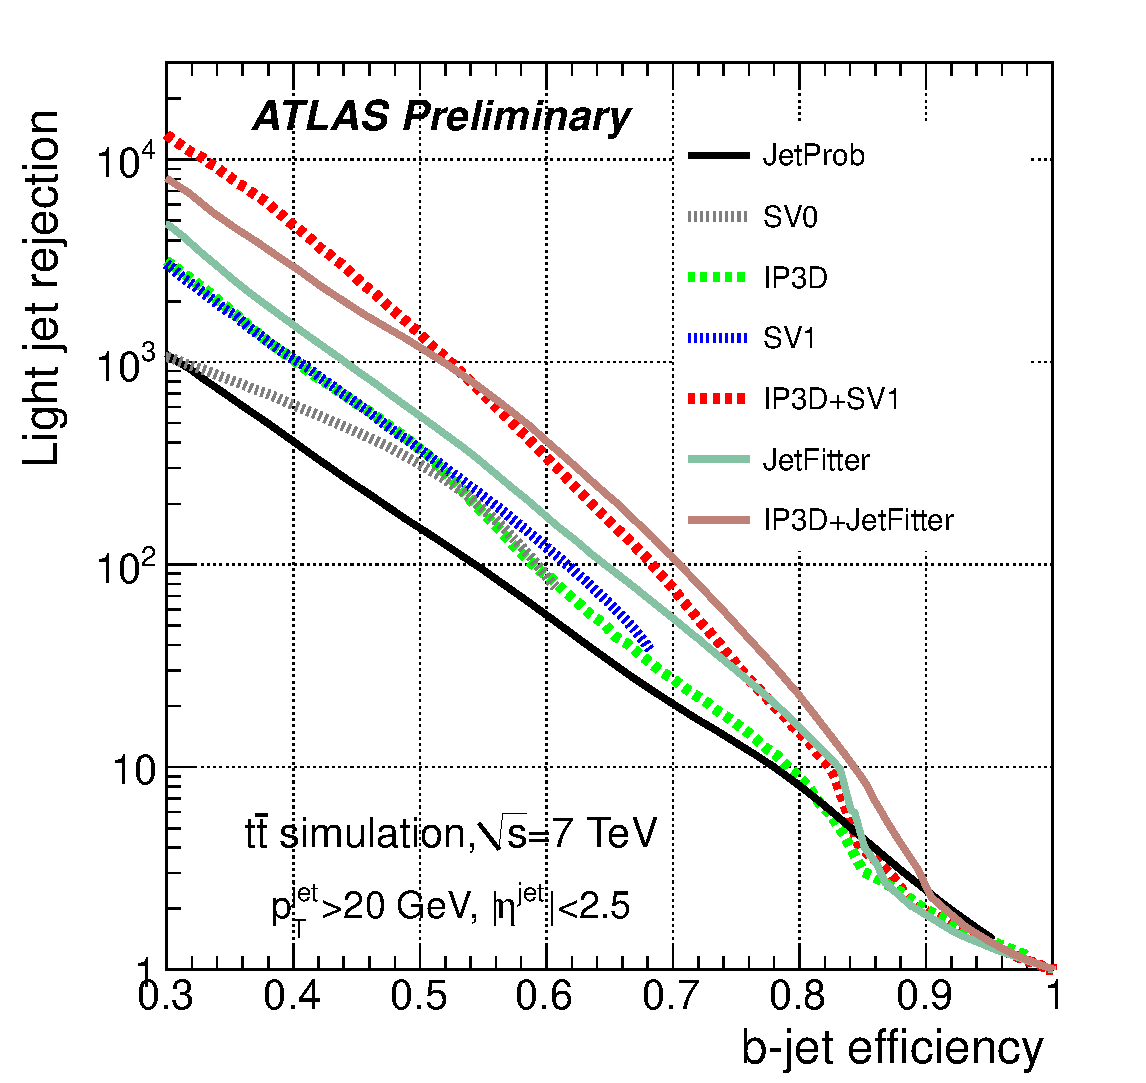
\includegraphics[width=0.6\textwidth]{figure/obj/btag_perf.pdf}

    \end{center}
    \caption{Light-jet rejection as a function of the b-jet tagging efficiency for several different tagging algorithms~\cite{btagPerf},
	obtained with simulated $\ttbar$ events. The rejection is defined as the inverse of mistagging rate of light jets.}
   \label{fig:beff}
\end{figure}

The performance of the mentioned algorithms is evaluated in data selecting $\ttbar$ events and compared to simulation~\cite{btagPerf}.
Figure~\ref{fig:beff} shows the b-tagging efficiency as a function of the inverse of the light-jet mistagging rate
for different b-tagging algorithm on $\ttbar$ simulated events. The tagging efficiency $\epsilon_b^{\ttbar}$ obtained from $\ttbar$ events
is used to define several b-tagging working points. Corrections due to non perfect modelling
of the b-tagging performance are evaluated by means of several methods
in~\cite{BtaggingScaleFactors, BtaggingScaleFactorsNew} and used to determine event weights for simulated events.
The uncertainties on these corrections  range from 5-10\%  depending on the $\pt$ and pseudorapidity of the jet.


\section{Tau-Jet Reconstruction}\label{sec:tau}
The reconstruction of jets originating from hadronically decaying $\tau$ leptons (in the following $\tau$-jets)
is described in detail in~\cite{AtlasCSCBook}.
A $\tau$-jet candidate is seeded by reconstructed calorimeter jets with $\pt > 10$ GeV and $|\eta| < 2.5$.
Tracks are then associated to the jet and a combination of the tracking and calorimeter information
is performed.  $\tau$-jets    can be distinguished from other 
jets by their low track multiplicity and a narrower clustering of energy deposit in the electromagnetic and hadronic calorimeters.
 The $\tau$-jet identification in ATLAS is based on a Boosted Decision Trees (BDT) multivariate procedure~\cite{ATLASTAUIDnew}.
One BDT discriminant has been developed to discriminate $\tau$-jets  from quark and gluon 
initiated jets and a separate one was developed to reject electrons.


\section{Missing Transverse Energy } \label{sec:met}
The missing transverse energy, \met, is the the vectorial sum of the transverse momenta
of all the physics objects and calorimeter cells in the event changed of sign. 
Undetected particles, such as neutrinos, lead to an unbalance of the total
transverse momentum, thus, to a non zero value of \met.

Reconstruction and calibration of \met with the  ATLAS detector is described in detail in~\cite{ETMISS}. 
The missing transverse energy measurement relies on the reconstruction of all physics objects 
in the event, it includes: muons and their energy deposits in the calorimeter, electrons, jets (weighted by their corresponding JVF), 
inner detector tracks (to take into account low-$\pt$ particles which are not well reconstructed in the calorimeters),
photons and $\tau$ leptons. The calorimeters cells are calibrated depending on the
pjysics object with which they are associated. The transverse energy of cells not associated to any object is taken into account in 
the so called ``CellOut'' contribution. This contribution,  together with the one related to jets with $10 < \pt < 20$ GeV
are referred to as the \emph{soft term} of the missing transverse energy.
The soft term is found to be very sensitive to pile-up. In order to reduce the impact of pile-up, the soft term
is scaled  by  the corresponding soft-term-vertex-fraction (STVF), which is calculated in the same way as JVF for jets.

A detailed description of the performance of the  \met reconstruction and calibration may be found in~\cite{ETMISS2}.


\section{Overlap Removal} \label{sec:olr}
Reconstruction of  physics objects defined in the previous section may sometimes
be ambiguous. For example, a $\tau$-jet is always reconstructed also as a common jet.
To avoid double counting of the physics objects originating from the same particle, an overlap removal procedure
is performed. A match between physics object of different sort is seeded  in a cone of $\Delta R <0.2$.
If  the matching occurs, the object with the lowest ranking is removed from the event. 
Physics object are ranked according to the following order, starting with the highest rank: muon, electron, $\tau$-jet 
and finally common jets.

\section{Trigger}
The ATLAS trigger system~\cite{trigger} consists of three stages. The Level-1 (L1) trigger is an
hardware trigger which reduces the event rate to approximatively 100 kHz and selects the Regions of
Interest (RoI) to be further investigated by the High Level Trigger (HLT). The HLT
comprises the Level-2 (L2) trigger employing fast reconstruction algorithms and the
Event Filter (EF) exploiting the full ATLAS event reconstruction.

In the presented search two triggers are employed: an electron EF trigger, which selects events containing 
an electron with $\pt >24 $~GeV and a combined muon-electron EF trigger, which requires the presence of a muon with $\pt > 8$~GeV and 
an electron with $\pt > 12$~GeV in the event. Detailed description of the muon and electron triggers can be found in~\cite{triggermu,triggere}.
Trigger efficiency for both triggers is evaluated in data selecting $Z$ candidate events and compared with prediction from simulation. Corrections are derived 
as function of the lepton pseudorapidity and transverse  momentum to match the simulated  trigger efficiency 
with the one in  data~\cite{triggermu,triggere}.

\section{Truth Particles}
For simulated events, the ATLAS reconstruction software provides information about the generated 
particles (called \emph{truth particles}). The irrticle type, the kinematic properties, decays and 
interactions are recorded following the conventions  in~\cite{hepmc}.
A particle is defined as stable if $c \tau > 1$~m, where $\tau$ is its mean life time. Particles emerging from 
interactions in the detector are excluded from this definition. 
Each particle in the event has a unique identifier (so-called ``bar-code''). 
Jets reconstructed from stable particles are called \emph{truth jets}.























